% !TEX root = main.tex

\section{Context and scope of the project}
\subsection{Context and Problem formulation}

Nowadays one of the most extensive uses of computing is artificial intelligence. This is being
used from, based on our preferences, help us select what products we can buy to properly detect
and focus faces when taking a picture. The main advantage of this field is that it reduces the
amount of human intervention and it usually performs better.

Inside AI one of the domains that has greatly increased during the last years is 
\emph{Machine Learning}. The main advantage is that it can solely learn from examples without 
explicit teaching, and thus reducing the human interaction during the learning process. One of the 
most used types is \emph{deep neural networks} and these have demonstrated impressive performance 
against tasks like the classification of digits from the MNIST data set.
~\cites{MNIST}{empirical-evaluation-deep-architectures}

Regarding the medical field, recent deep learning algorithms, specially convolutional networks 
have started to push the boundaries of precision medicine. 
Traditionally, medical predictions have been based on a few clinical parameters with poor accuracy.
However, other data types are available to improve such predictions. In this context, medical
images generated from MRI, PET or CT scans are vastly underused due to the inability of radiologists
to quantitatively analyze this complex data.

Different methods have appeared to analyze these images for tasks such as
image classification, object detection, segmentation and registration among other tasks. This
approach started in the late 1990s and has slowly shifted from systems that are completely designed
by humans to systems that are trained by computers using example data. 
~\cite{survey-deep-learning}

Professor Benjamin Haibe-Kains has helped in the development of \emph{Radiomics}, a new field to
relying on pre-defined, hand-engineered features computed from medical images to better 
characterize tumours and predict survival outcome. Although promising, radiomics suffers from 
two several limitations: the number of features is limited and it is a slow process as it requires
a radiologist to manually contour the tumour. Deep learning has the potential to address both issues
by automatically extract more information from the images.
~\cite{radiomics-ML-classifiers}

To use all this data, Survival Prediction models have been created. This type of models are
used to understand the relations between patients and effectiveness of various treatment options. 
The survival and hazard functions are the two fundamental functions in survival analysis. The
survival function \( S(t) = \Pr(T > t) \), is the probability that an individual has
\emph{survived} beyond time \( t \). The hazard function \( \lambda(t) \) is a measure of risk at 
time \( t \) and it's defined as:
~\cite{DeepSurv}
\[
    \lambda(t) = \lim_{\delta \rightarrow 0}
    \frac{\Pr(t \le T < t + \delta | T \ge t)}{\delta}
\]


Also, to compare if an algorithm is performing better than another one we usually use the ROC curve
which compares the \emph{False Positive Rate} against the \emph{True Positive Rate}, see 
\autoref{fig:ROC-curve}. The Cox Proportional Hazards (CPH) model provides a starting point for a 
survival model and the future models will be compared against this one.
~\cites{ROC-precision-recall}{Cox}

\begin{figure}
    \centering
    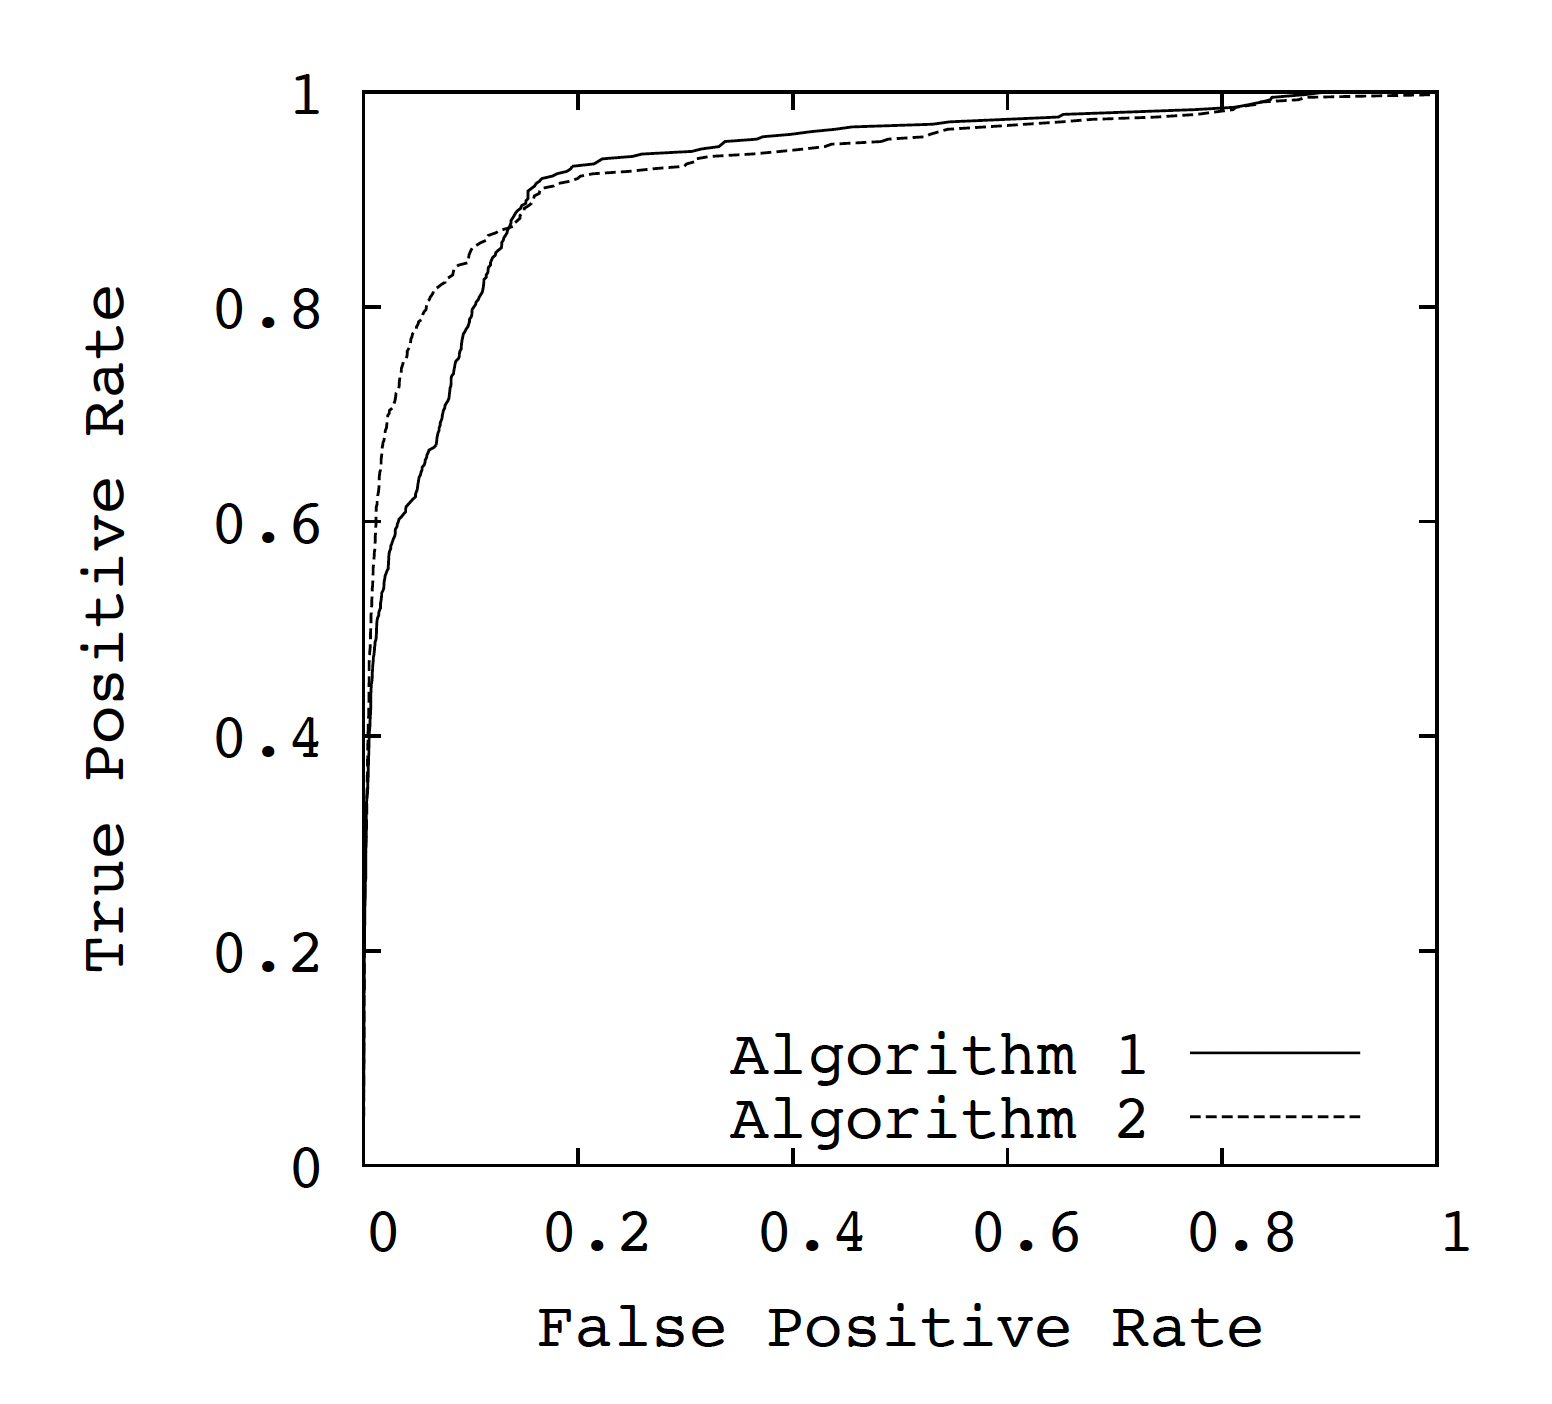
\includegraphics[width=.5\linewidth]{images/roc_curve}
    \caption{ROC Curve example\label{fig:ROC-curve}}
\end{figure}

Through a collaboration with Dr.~Fei-Fei Liu, head of the Radiation Medicine Program at Princess
Margaret Cancer Centre, prof. Benjamin Haibe-Kains has access to a unique set of \( {\sim}500 \) 
scans of head-and-neck cancer patients with associated survival data. The goal of this project is 
to develop a new deep learning framework to analyze this private dataset in combination with public 
databases to improve the prediction rate of patients' survival compared to models built on 
traditional radiomic features. Two of the methods that will be explored are dropout and image 
augmentation techniques to improve the fitting of neural networks from medical images. 

\subsection{State-of-the-art}

A lot of research is being done in the medical field using deep learning during these days. Image
classification is one of the first areas in which there's a major contribution to medical analysis.
Usually in image classification one has one or multiple images as input and a single diagnostic 
variable as output (e.g.~ill or not). With this approach the use of transfer learning has been a
great improvement.
~\cite{survey-deep-learning}

Through transfer learning is the use of pre-trained networks to try to reduce the requirement of 
large data sets for deep network training. Usually there are two possible strategies: (1) using a 
pre-trained NN as a feature extractor and (2) fine-tuning a pre-trained network on medical data.
Both strategies are popular and have been widely applied. One of the networks that allow this type
of retrain is GoogLeNet Inception v3.
~\cites{GoogLeNet}{NNRetrain}{inceptionRetrain}

Moreover, regarding the prediction of survival models there have been different approaches but
almost all of them use MRI, PET or CT scans and the medical records. The typical one is to extract
hand-crafted radiomic features using own methods or using libraries such as
\href{https://github.com/Radiomics/pyradiomics}{\emph{PyRadiomics}}. This hand-crafted features are
based in things like tumour shape intensity, shape or texture.
~\cites{PyRadiomics}{tumour-radiomics}

The other approach is using a deep learning-based model for prediction. In this case too, 
hand-crafted features are extracted but besides a Convolutional Neural Network is used to extract
features. So this way the number of extracted features is bigger. There's the problem that when
extracting hand-crafted features from a CT scan this is a 3D image while when working with a 
CNN only 2D images can be used, since there's still no pre-trained CNN on 3D images. Although
this method seems promising still requires further work to train a dedicated feature extractor 
explicitly designed for medical images.
~\cite{deep-learning-radiomics-gbm}

An implemented survival prediction model is \emph{DeepSurv} which based on survival data,
comprised of three elements: patient's baseline data, failure event time and an event indicator.
\emph{DeepSurv} is an Open Source Python module that applies recent deep learning techniques to
a nonlinear Cox proportional hazards network. 
~\cite{DeepSurv}

\subsection{Scope}

The first task will be learning and understanding how Neural Networks and specifically how 
Convolutional Neural Networks Work. This way I will have a fully understanding of the background
that all this methods use create models for survival prediction.

The next task will be setting up and running the \emph{DeepSurv} python package on a local computer.
This will mean trying to test all the methods that can be used and see which parts can be reused 
to create a new Survival Prediction Model. Since this model does not seem to be adapted for images
as input then an improvement will be focused in trying to pass medical images as input to train
the survival model. Once this task is finished then th results will be compared to less complex
survival methods such as random survival forests.

An extension of the previous task will be to convert the survival problem with head-and-neck data
to a binary classification problem and implement different CNN architectures (starting from 
shallow to deep). Performance measurements will be important and also prevent overfitting, since 
this can lead to wrong results, to ensure a successful training.

\subsection{Methodology}

This project is part of a research project at Benjamin Haibe-Kains Bioinformatics and 
Computational Genomics Laboratory. This means that every week there will be a laboratory meeting
where progress will be presented to all the lab members and feedback will be received accordingly. 

Also since there are different ways of development this means that it will have a process of trial
and error until the proper solution is found. This means that during this process the
tasks will be assigned on a weekly basis.
